\chapter{Current Wireless Systems}
We now present a brief review of some of the most commonly used wireless 
systems.

\section{Cellular Systems}
Cellular Systems are based on cells. Each cell has a different signal 
from the ones in its immediate vicinity to allow for seamless transitions (see 
the different colors in Figure~\ref{fig:cws:CellSys}). Frequencies, time 
slots and codes are reused at spacially-separated locations. At the center of 
each cell there is an antenna, certain antennas are more powerful than others 
and can manage hand-offs and control functions. These antennas are called Base 
Stations. Hand-offs can be can be horizontal if they occur between the same 
technology (4G$\to$4G) or vertical otherwise 
(3G$\leftrightarrow$4G).
Having larger cells means having lesser transitions but also more people 
accessing the same cell. If there are too many people and there isn't enough 
bandwidth you won't be able to use your device. Shrinking cell size increases 
capacity, as well as networking burden
\begin{figure}[!h]
  \centering
  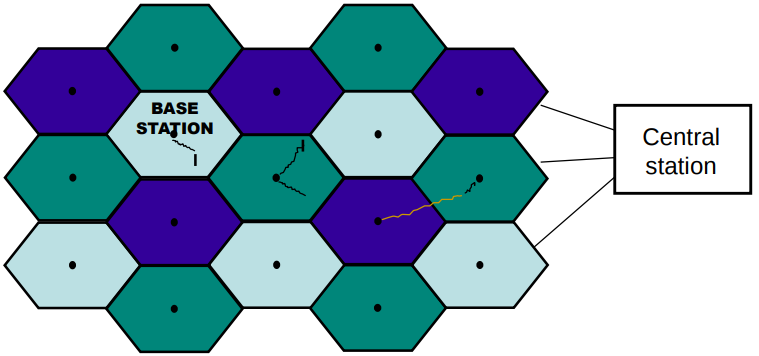
\includegraphics[width=0.8\linewidth]{CellSys.png}
  \caption{Cellular Systems}				
  \label{fig:cws:CellSys}
\end{figure}

\section{Wireless Local Area Networks (WLAN)}
WLAN is used to connect local computers (within 100m range). We have an 
access point, connected to the Internet through a wire and using protocol 
802.11. The access point not only forwards data, it also coordinates users and 
breaks data into packets. In fact, even though data arrives already broken, 
access points break it further, because the smaller the packet transmitted, the 
better. Obviously, this becomes a problem when we relate it to overhead: since 
overhead has a fixed size, independent from the packet's size, we may find 
ourselves in the situation where, faced with $1000\ data + 40\ overhead$ we end
up with $500\ data + 40\ overhead$ plus $500\ data + 40\ overhead$.
We still prefer splitting, because, when facing a big error rate we 
don't want to lose all the packets.
The WLAN channel access is shared using random access and this system 
forms the backbone of current Internet, providing a best-effort service.

\begin{figure}[t]
  \centering
  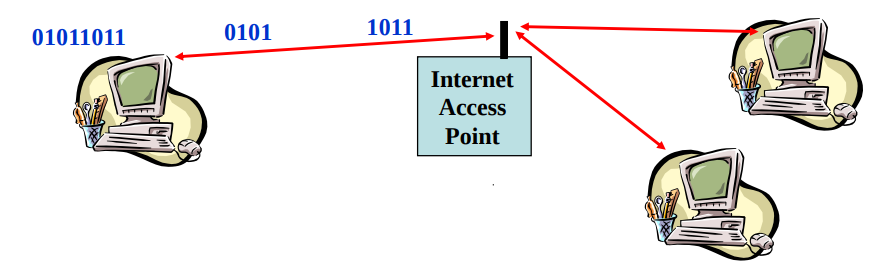
\includegraphics[width=0.8\linewidth]{WLAN.png}
  \caption{Wireless Local Area Networks (WLAN)}			
  
  \label{fig:cws:WLAN}
\end{figure}

\paragraph*{Wireless LAN Standards}
See overview in Table~\ref{tab:cws:WLANStd}.
\begin{table}[b]
\centering
\begin{tabular}{l|l|l|l|l|}
\cline{2-5}
&\textbf{802.11b}     & \textbf{802.11g}     & \textbf{802.11n}     & \textbf{802.11ac}    \\ \hline
\textbf{Frequency}    &2.4GHz   & 2.4GHz/5GHz & 2.4GHz/5GHz & 2.4GHz/5GHz \\ \hline
\textbf{Bandwidth}    &1-11Mbps & 54Mbps      & 300Mbps     & 500Mbps     \\ \hline
\textbf{Add. features}&         & OFDM        & MIMO        & MIMO        \\ \hline
\end{tabular}
\caption{Wireless LAN Standards}
\label{tab:cws:WLANStd}
\end{table}


Note that:
\begin{itemize}
\item 802.11b is a free frequency and therefore crowded
\item 802.11g is quite popular, using a higher bandwidth. It 
  brought changes in the physical layer.
\item 802.11n MIMO (Multiple-Input and Multiple-Output). A 
  device using this standard can be easily recognized because it uses multiple 
  antennas and multiple channels.
\end{itemize}

\section{Satellite Systems}
They are used to cover very large areas. There exist two types of 
satellites that have different orbit heights: GEO satellites (GEOstationary) 
stay at about 39000 km while LEO satellites (Low Earth Orbit) stay lower, at 
2000 km. GEO are so high that remain stationary and can cover the whole surface 
while LEO revolve continuously in order not to fall.
Satellites are usually a two way system, optimize for one-way 
transmission: usually satellite $\to$ earth is faster than the other way.

\section{Bluetooth}
Bluetooth was invented as a cable replacement, and this is why it is 
short-range (about 10 m). The band used (2.3 GHz) is crowded but cheap, and 
Bluetooth originally has one data and three voice channels.
One other reason why the range is so short is to avoid consuming too much 
battery. Also, note that the signal strength decreases exponentially and not 
linearly with the distance.


